\documentclass[12pt]{article}
\usepackage[utf8]{inputenc}
\usepackage[italian]{babel}
\usepackage{amsmath}
\usepackage{longtable}
\usepackage{graphicx}
\usepackage{amssymb}
\usepackage{float}
\usepackage{listings}
\usepackage{color}
\usepackage{hyperref}

\lstloadlanguages{C,C++,csh,Java}

\definecolor{red}{rgb}{0.6,0,0} 
\definecolor{blue}{rgb}{0,0,0.6}
\definecolor{green}{rgb}{0,0.8,0}
\definecolor{cyan}{rgb}{0.0,0.6,0.6}
\definecolor{cloudwhite}{rgb}{0.9412, 0.9608, 0.8471}

\lstset{
language=csh,
basicstyle=\footnotesize\ttfamily,
numbers=left,
numberstyle=\tiny,
numbersep=5pt,
tabsize=2,
extendedchars=true,
breaklines=true,
frame=b,
stringstyle=\color{blue}\ttfamily,
showspaces=false,
showtabs=false,
xleftmargin=17pt,
framexleftmargin=17pt,
framexrightmargin=5pt,
framexbottommargin=4pt,
commentstyle=\color{green},
morecomment=[l]{//},
morecomment=[s]{/*}{*/},
showstringspaces=false,
morekeywords={ abstract, event, new, struct,
as, explicit, null, switch,
base, extern, object, this,
bool, false, operator, throw,
break, finally, out, true,
byte, fixed, override, try,
case, float, params, typeof,
catch, for, private, uint,
char, foreach, protected, ulong,
checked, goto, public, unchecked,
class, if, readonly, unsafe,
const, implicit, ref, ushort,
continue, in, return, using,
decimal, int, sbyte, virtual,
default, interface, sealed, volatile,
delegate, internal, short, void,
do, is, sizeof, while,
double, lock, stackalloc,
else, long, static,
enum, namespace, string},
keywordstyle=\color{cyan},
identifierstyle=\color{red},
backgroundcolor=\color{cloudwhite},
}

\usepackage{caption}
\DeclareCaptionFont{white}{\color{white}}
\DeclareCaptionFormat{listing}{\colorbox{blue}{\parbox{\textwidth}{\hspace{15pt}#1#2#3}}}
\captionsetup[lstlisting]{format=listing,labelfont=white,textfont=white, singlelinecheck=false, margin=0pt, font={bf,footnotesize}}

\newcommand*{\ditto}{\texttt{"}}

\graphicspath{ {./images/} }

\title{Ingegneria del software - Memory e Dama Multiplayer}
\author{Fabrizio Corriera}
\date{2019/2020}

\begin{document}

\maketitle
\thispagestyle{empty}
\newpage
\pagenumbering{roman}
\tableofcontents
\newpage
\pagenumbering{arabic}

\section{Introduzione}

\subsection{Obiettivo}
L'obiettivo di questo documento consiste nel fornire una panoramica completa sul processo di pianificazione, analisi dei requisiti funzionali, studio delle risorse e sviluppo di un software utilizzando una strategia di tipo agile.
Il software in questione è un tool che presenta all'interno sia un videogioco 3D che ripropone il classico gioco da tavolo della dama con la possibilità di giocare con altri giocatori in locale o online, sia un videogioco 3D che ripropone il classico gioco del memory in locale tra due giocatori.

\subsection{Solo Extreme Programming}
Ho deciso di utilizzare una metodologia agile simile all'Extreme Programming (XP) ma adattata al lavoro in solitario.
L'XP è una metodologia di sviluppo software di tipo agile che pone enfasi sul lavoro di squadra e segue 12 regole fondamentali, divise in 4 categorie:

\begin{itemize}
\item \textbf{Feedback a scala fine}
	\begin{itemize}
	\item Pair programming: lavorando in due sulla stessa macchina al medesimo codice, il prodotto sarà di qualità superiore.
	\item Planning game: una riunione di pianificazione che avviene ad ogni iterazione (circa una volta a settimana).
	\item Test driven development: test automatici scritti prima di scrivere il codice.
	\item Whole team: il cliente deve essere presente e disponibile a verificare la qualità e la funzionalità del prodotto.
	\end{itemize}
\item \textbf{Processo continuo}
	\begin{itemize}
	\item Integrazione continua: integrare continuamente i cambiamenti al codice eviterà ritardi più avanti nel ciclo del progetto.
	\item Refactoring: riscrivere il codice senza alterarne le funzionalità esterne, in modo da renderlo più semplice e generico.
	\item Small releases: frequenti rilasci di funzionalità.
	\end{itemize}
\item \textbf{Comprensione condivisa}
	\begin{itemize}
	\item Coding standards: scrivere il codice seguendo uno standard di regole ben definite da tutto il team.
	\item Collective code ownership: ognuno è egualmente responsabile della totalità del codice.
	\item Simple design: sia nei confronti del codice che del cliente i programmatori dovrebbero mantenere un approccio orientato alla semplicità.
	\item System metaphor: il sistema ed il suo funzionamento dovrebbero essere descritti con una metafora.
	\end{itemize}
\item \textbf{Benessere dei programmatori}
	\begin{itemize}
	\item Sustainable pace: la cosiddetta 40-hour week; nessuno nel team dovrebbe lavorare più di 40 ore a settimana.
	\end{itemize}
\end{itemize}

\begin{figure}[H]
\centering
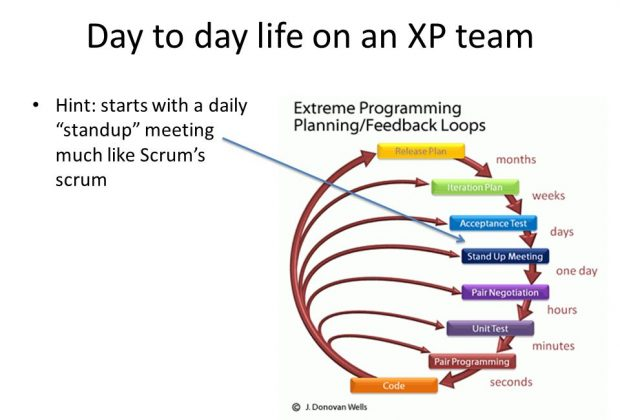
\includegraphics[scale=.5]{XP}
\caption{Rappresentazione del loop che definisce il lavoro di un team che usa XP}
\label{img:XP}
\end{figure}

Ovviamente nel caso di un progetto sviluppato da un team composto da un'unica persona (come quello descritto in quella relazione), alcune regole perdono di significato: sicuramente il pair programming non è possibile, seppure sia possibile ottenere comunque un altro punto di vista sul proprio codice attraverso il rubber duck debugging, e l'integrazione risulta costantemente immediata, a meno che non si lavori su più branch.

Generalmente si utilizzano le "user stories", delle descrizioni ad alto livello delle funzionalità del software che permettono di dividere il lavoro in blocchi logici, focalizzandosi sul risultato da dover ottenere. Le stories vanno scritte con un linguaggio molto semplice, senza la necessità di specificare dei requisiti che verranno descritti in seguito. Inoltre è fondamentale fare periodicamente dei test sull'accettabilità del codice, concordandone i criteri con il cliente.

Anche un unico programmatore può mantenere costanti le release del software: dividendo il progetto in diverse iterazioni e pianificandole di volta in volta. Resta comunque fondamentale la focalizzazione sulla comunicazione ed il feedback con il cliente (due elementi chiave nell'XP). Una trappola molto comune in cui è possibile cascare è cercare di lavorare più duramente o al lungo per mettersi in pari con la scaletta originale. Invece è sempre meglio, secondo la filosofia dell'XP, fare un nuovo "planning meeting", tirare le somme, accettare dove si è arrivati e studiare un nuovo piano di azione.

A tal proposito è infatti estremamente importante mantenere un andamento costante e sostenibile. Anziché condurre degli stand-up privati, più semplicemente è possibile dedicare un momento ogni giorno alla gestione degli imprevisti e allo scopo di riottenere il focus sul lavoro.

Utilizzare un design semplice ed una metafora per il sistema è quantomai fondamentale anche lavorando da soli. Assegnare la responsabilità alle classi e agli oggetti usando dei pattern GRASP (General Responsibility Assignment Software Patterns) piuttosto che delle carte CRC (Class Responsibility Collaboration) può essere d'aiuto in tal senso.

Lavorare iterativamente senza mai mostrare i risultati al cliente è un errore da evitare. In tal senso avrebbe addirittura senso pensare di lavorare faccia a faccia con il cliente per migliorare la comunicazione con quest'ultimo.

Anche se si lavora da soli è necessario stabilire e mantenere degli standard nella stesura del codice. Ciò renderà il codice molto più leggibile, comprensibile e facile da approcciare per il debug.

Se possibile potrebbe essere necessario testare il codice su più di una macchina. Non è detto che il funzionamento del software sia consistente se è stato testato su un'unica macchina.

Infine, ovviamente tutto il codice deve aver passato positivamente tutti i test prima della release. Se viene trovato un bug bisogna creare dei test a riguardo.

\subsection{Descrizione delle funzionalità del software}
Il software che desideriamo implementare consiste nella possibilità di scegliere tra giocare ad una rappresentazione 3D del gioco della dama, arricchita da una funzionalità multiplayer online e da una chat in-game o ad una rappresentazione 3D del gioco del memory. Ci aspettiamo che il software alla sua inizializzazione presenti un menù principale, con una grafica semplice ma d'impatto, e delle scelte da poter effettuare, ovvero:

\begin{enumerate}
\item Scegliere tra Memory e Dama Multiplayer
\item Iniziare una partita a Memory in locale contro un altro giocatore
\item Iniziare una partita a Dama in locale contro un altro giocatore.
\item Creare una stanza in cui ospitare una partita online di Dama.
\item Entrare in una stanza già esistente ed unirsi ad una partita online di Dama.
\end{enumerate}

Dal menù della Dama si potrà anche inserire lo username con cui venire identificati durante le partite multiplayer (in caso di input vuoto si verrà identificati come host se si sta ospitando la partita o client se si è ospiti nella stanza di un altro giocatore).

Se si sceglie una partita in locale, due giocatori potranno confrontarsi giocando sulla stessa macchina e la partità inizierà subito dopo aver selezionato l'opzione dal menù.

Se si sceglie di creare una stanza per ospitare una partita si verrà messi in attesa di un giocatore che si unisca alla stanza e si potrà sempre avere la possibilità di annullare e tornare indietro al menù principale.

Se si sceglie di unirsi ad un'altra partita verrà chiesto di inserire l'indirizzo IP del giocatore che sta correntemente attendendo che qualcuno entri nella sua stanza. Di dafault sarà inserito l'indirizzo locale (127.0.0.1), ma sarà possibile modificarlo e poi si dovrà selezionare la conferma dell'indirizzo o di tornare indietro al menù principale.

Nel momento in cui inizia una partita qualunque vogliamo che il gioco della dama venga rappresentato fedelmente: su una scacchiera 8x8 composta da un'alternanza di quadrati neri e bianchi ci sono 12 pedine nere e 12 bianche, situate ai due capi della scacchiera, posizionate solo sui quadrati neri. Le pedine possono essere mosse solo in avanti e in diagonale ed ovviamente non possono uscire dai limiti della scacchiera. Inizia il giocatore che muove le pedine bianche e ci aspettiamo che dopo che egli abbia mosso il turno passi al giocatore che muove le pedine nere e così via. Se una pedina si trova in una posizione adiacente ad una pedina avversaria, e la posizione seguente lungo la diagonale non è occupata, essa potrà e dovrà mangiare la pedina avversaria in questione: ciò vuol dire che si sposterà di due posizioni (fino ad occupare la poszione dietro la pedina "mangiata") e la pedina che è stata così scavalcata viene eliminata dal gioco. Se la pedina mossa ha mangiato e si trova in posizione di mangiare un'altra volta, il giocatore potrà e dovrà farlo prima di passare il turno; questo è l'unico caso in cui durante il proprio turno un giocatore muove più di una volta. Se una pedina raggiunge il limite avversario della scacchiera viene promossa e diventa una regina (re in inglese): ciò vuol dire che la suddetta pedina potrà muoversi in ambo le direzioni della scacchiera, mantenendo comunque la restrizione del movimento diagonale. Quando l'ultima pedina avversaria verrà mangiata, il giocatore che finisce il turno avrà vinto la partita.

Vogliamo che venga fatto presente di chi è il turno attuale, e che venga segnalato il vincitore. Inoltre intendiamo mettere un'evidenziazione dei pezzi che sono costretti a muovere in una determinata situazione. Ed infine, una volta conclusa la partita, il giocatore dovrà essere riportato al menù.

Durante la partita online sarà anche presente una chat in cui i due giocatori potranno scambiarsi messaggi in tempo reale mentre giocano. Nella chat sarà possibile scorrere i messaggi precedenti per leggerli o scriverne uno nuovo nell'apposita casella di input per poi inviarlo cliccando l'apposito tasto. I mittenti dei messaggi saranno evidenziati nella chat, in quanto i messaggi avranno un formato del tipo "Username: messaggio".

Quando inizia una partita di Memory vogliamo che vengano sistemate 20 coppie di carte coperte sul tavolo da gioco in ordine casuale, e che i giocatori, durante il loro turno, possano girare due carte. Se queste due carte sono uguali tra loro, quel giocatore ottiene 1 punto e potrà continuare a scoprire le carte. Se la coppia di carte girate non corrisponde, il giocatore dovrà rigirarle e passare il turno.

\subsection{Analisi dei requisiti}
Da questa breve descrizione possiamo individuare i requisiti di sistema del software, dividendoli in requisiti funzionali (descrivono ciò che il sistema dovrebbe fare) e requisiti non funzionali (non riguardano direttamente le funzioni fornite dal sistema ma ne specificano il comportamento, le politiche di organizzazione e sviluppo ecc). Partendo da questi requisiti scriveremo le User Stories che utilizzeremo durante lo sviluppo del progetto e che ci permetteranno di dividere il lavoro in maniera logica e incrementale.

\begin{itemize}
\item \textbf{Requisiti funzionali}
\begin{itemize}
\item Menù principale dove è possibile scegliere tra Dama e Memory.
\item Menù del Memory da dove si può procedere verso una partita locale con un altro giocatore o tornare indietro.
\item Menù della Dama da dove si può procedere verso: partita locale, hosting di una partita, entrare in una stanza esistente o tornare indietro.
\item Possibilità di definizione di uno username personalizzato.
\item Sottomenù di hosting.
\item Sottomenù di accesso ad una partita.
\item Partita locale.
\item Partita online.
\item Chat online.
\item Ritorno al menù principale dopo la vittoria di un giocatore.
\end{itemize}
\item \textbf{Requisiti non funzionali}
\begin{itemize}
\item Il gioco deve essere 3D.
\item Il progetto deve essere sviluppato con il motore grafico Unity.
\item Il progetto deve usare il linguaggio di programmazione C\#.
\item La funzionalità online deve usare il protocollo TCP senza ausilio di tool esterni.
\item La metodologia di sviluppo del software deve essere XP.
\item La consegna del software con annessa documentazione deve avvenire entro la data 02/09/2020.
\end{itemize}
\end{itemize}

\subsection{Diagrammi dei casi d'uso}
Presentiamo qui di seguito i diagrammi dei casi d'uso, o diagrammi use case, del nostro software. Un diagramma use case è un diagramma UML che viene usato per descrivere un set di azioni o funzionalità che un sistema può o dovrebbe svolgere con l'ausilio di uno o più utenti esterni.

Qui di seguito vediamo la traduzione in diagrammi use case di quanto è stato detto finora descrivendo le funzionalità del nostro software:

\begin{figure}[H]
\centering
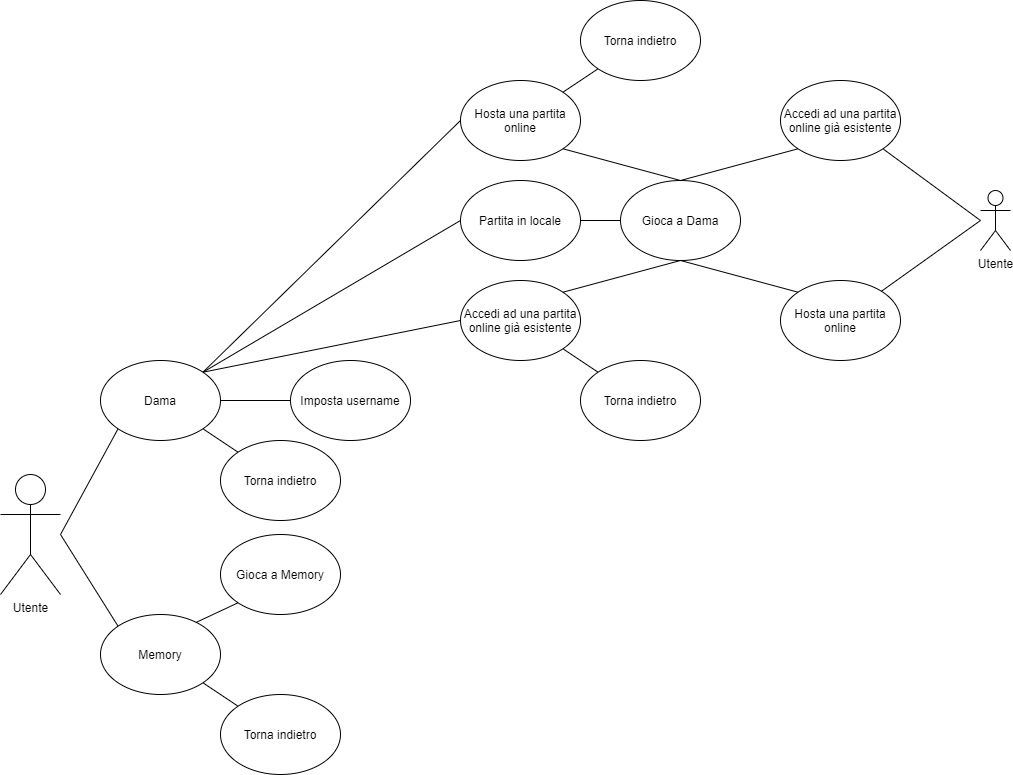
\includegraphics[scale=.35]{UseCaseMain}
\caption{Diagramma Use Case del menù di gioco}
\label{img:usecasemain}
\end{figure}

Nella figura \ref{img:usecasemain} è rappresentato il diagramma dei casi d'uso in riferimento al menù principale del software che ci accingiamo a sviluppare, e da qui possiamo vedere che l'utente al momento dell'avvio del programma può scegliere tra accedere al sottomenù della Dama e accedere al sottomenù del Memory.

Nel primo caso avrà davanti a se la possibilità di impostare uno username, tornare al menù precedente o di scegliere la modalità di gioco tra quelle proposte: locale oppure online con il ruolo di host o di guest (in questi ultimi due casi, come è possibile vedere, servirà l'ausilio di un ulteriore utente per poter avviare una partita di dama).

Nel secondo caso potrà scegliere tra avviare una partita a Memory o tornare al menù precedente.

\begin{figure}[H]
\centering
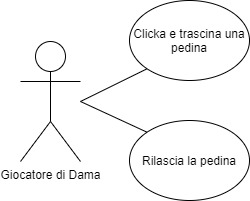
\includegraphics[scale=.5]{UseCaseCheckers}
\caption{Diagramma Use Case di una partita in locale a Dama}
\label{img:usecasecheckers}
\end{figure}

L'utente, una volta che avvierà una partita di Dama, verrà riconosciuto come Giocatore di Dama, una generalizzazione del caso utente. Egli all'interno della partita di Dama potrà selezionare col click del mouse e la pressione continua del tasto sia il pezzo da muovere che la sua destinazione, trascinandolo verso di essa; oppure, rilasciando un pezzo della scacchiera già selezionato, potrà deselezionarlo o muoverlo.

\begin{figure}[H]
\centering
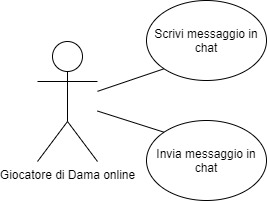
\includegraphics[scale=.5]{UseCaseCheckersMultiplayer}
\caption{Diagramma Use Case di una partita online a Dama}
\label{img:usecasecheckers}
\end{figure}

Nel caso di una partita online a Dama, il Giocatore di Dama Online, generalizzazione del Giocatore di Dama, potrà scrivere dei messaggi in chat ed inviarli.

\begin{figure}[H]
\centering
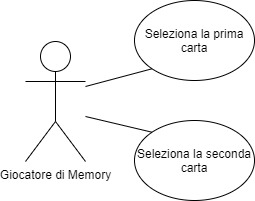
\includegraphics[scale=.5]{UseCaseMemory}
\caption{Diagramma Use Case di una partita a Memory}
\label{img:usecasememory}
\end{figure}

Nel caso invece di una partita a Memory, chiameremo la generalizzazione dell'Utente, Giocatore di Memory, ed egli, una volta avviata la partita di Memory, potrà selezionare la prima carta del suo turno e la seconda.

\begin{figure}[H]
\centering
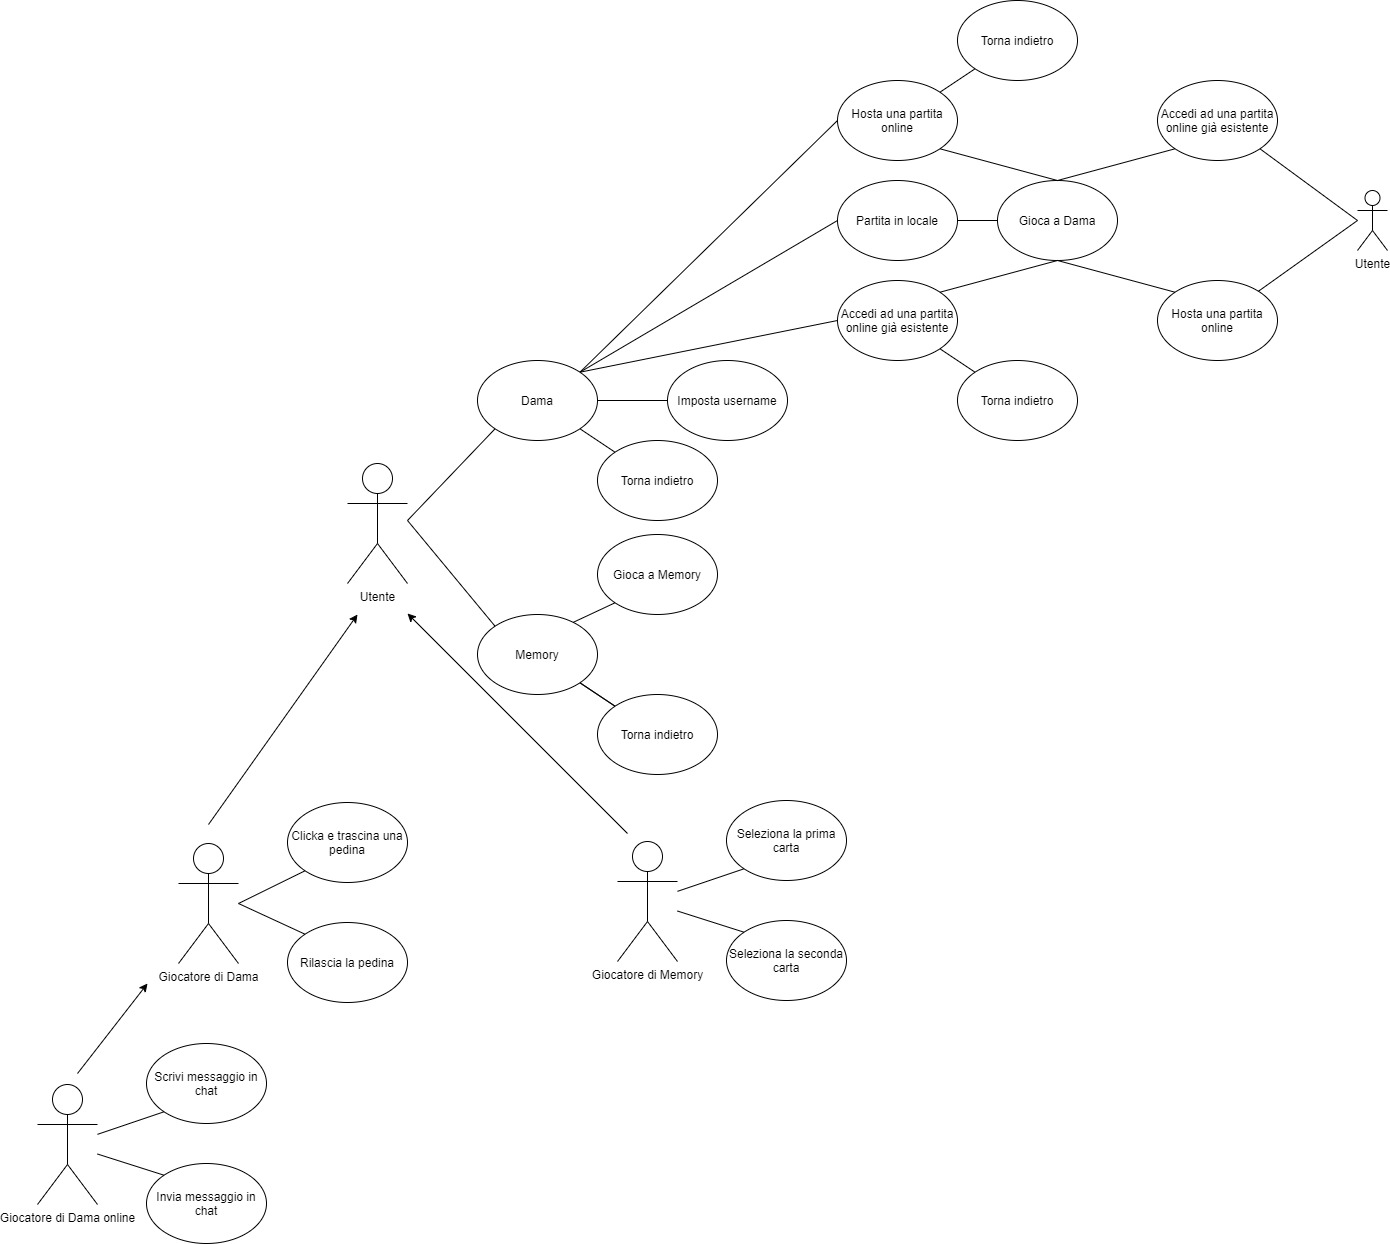
\includegraphics[scale=.3]{UseCaseGeneral}
\caption{Diagramma Use Case generale del software}
\label{img:usecasegeneral}
\end{figure}

Nella figura \ref{img:usecasegeneral} possiamo vedere il diagramma Use Case completo del software, dove gli attori e le loro generalizzazioni sono collegati tra loro ed è possibile vedere una panoramica completa dei casi d'uso del progetto.

\section{Sviluppo del software}
In questa parte del documento verrà trattato tutto il processo di sviluppo del software discutendone gli strumenti, l'organizzazione, le strategie, i metodi e valutandone infine i risultati.

\subsection{Strumenti utilizzati}
Nello sviluppo di questo software sono stati impiegati i seguenti strumenti:

\begin{itemize}
\item{\textbf{Unity:}} Unity è un motore grafico multipiattaforma sviluppato da Unity Technologies che consente lo sviluppo di videogiochi e altri contenuti interattivi, quali visualizzazioni architettoniche o animazioni 3D in tempo reale. La scelta è ricaduta su Unity piuttosto che sugli altri concorrenti sul mercato in quanto esso offre un piano gratuito completo di ogni funzionalità, avevo già delle esperienze di programmazione in C\# e soprattutto, al momento della scrittura di questo documento (Agosto 2020), Unity è uno dei motori grafici più utilizzati nel panorama professionale dello sviluppo di videogiochi.
\item{\textbf{Microsoft Visual Studio:}} Microsoft Visual Studio (o più comunemente Visual Studio) è un ambiente di sviluppo integrato (Integrated development environment o IDE) sviluppato da Microsoft. In questo caso la scelta è stata quasi ovvia, in quanto l'integrazione tra Unity e Visual Studio è totalmente supportata dai loro sviluppatori.
\item{\textbf{\LaTeX:}} \LaTeX è un linguaggio di markup per la preparazione di testi, basato sul programma di composizione tipografica \TeX ed è stato utilizzato per la scrittura di questo documento.
\item{\textbf{Asset grafici gratuiti:}} Alcuni asset grafici utilizzati in questo progetto sono asset gratuiti o con licenza freeware acquistati sull'asset store di Unity. Lo skybox e l'acqua utilizzati nella scenografia del gioco sono asset gratuiti utilizzati in maniera lecita secondo le norme delle loro licenze.
\item{\textbf{Draw.io:}} Draw.io è un'applicazione di diagrammi gratuita che è stata impiegata per disegnare tutti i diagrammi presenti in questo documento.
\end{itemize}

\subsection{Progettazione}
Suddividiamo il lavoro in maniera logica ed iterativa, individuando le caratteristiche del progetto che possono essere implementate in maniera "stand-alone", permettendoci quindi di poter sostenere delle release continue augurandoci un ritmo di almeno una release al giorno. Scriviamo quindi le user stories.
\newline

\textbf{\Large User stories 1}
\begin{enumerate}
\item Creazione scacchiera e pezzi
\item Codifica del movimento dei pezzi
\item Regole per il movimento dei pezzi
\item Codifica del codice per il check della validità delle mosse
\item Promozione a regina
\item Codifica lato server
\item Codifica lato client
\item Creazione Menù
\item Connessione utenti
\item Invio delle mosse online
\item Miglioramenti estetici e inserimento degli alert
\item Codifica della partita in locale
\item Effetti grafici per i pezzi costretti a muovere
\item Codifica della chat in-game
\item Abbellimenti grafici
\end{enumerate}

Questa lista è stata stilata nell'ordine in cui le stories sono state prese in carico e le funzionalità da loro descritte implementate. Non tutte esistono dai primi istanti di vita del progetto, infatti la 12, la 13 e la 14 sono state inserite in un secondo momento per far fronte a delle necessità, per favorire  lo sviluppo di altre funzionalità o in generale per migliorare il risultato finale del progetto.

A seguito della richiesta da parte del cliente dell'aggiunta di un secondo gioco (Memory) nel softwre, sono state aggiunte le seguenti storie:
\newline

\textbf{\Large User Stories 2}
\begin{enumerate}
\item Creazione tavolo e carte
\item Codifica delle regole di gioco
\item Codifica notifiche a schermo
\item Creazione menù Memory e menù principale
\item Perfezionamenti
\end{enumerate}

In questo caso le storie sono di numero molto inferiore perché dovranno essere esaurite in un tempo molto più ristretto, e ci si è basati maggiormente sulle macrofunzionalità di gioco, suddividendo così il progetto in poche ma grandi aree tematiche (ciò è stato reso possibile anche dalla maggiore semplicità del gioco da implementare).

\subsection{Sviluppo}
\begin{itemize}
\item \textbf{Inizio - 11/08/2020}
	\begin{itemize}
	\item \textbf{Inizio Storia 1}
	\item Creazione dei modelli 3D della scacchiera e dei pezzi
	\item Creazione e applicazione delle texture ai modelli 3D
	\item Creazione dello script CheckersBoard.cs
	\item Creazione dello script Piece.cs
	\item Generazione dei pedoni sulla scacchiera (metodi GenerateBoard, GeneratePiece e MovePiece dello script CheckersBoard.cs)
	\item \textbf{Fine Storia 1}
	\item \textbf{Release 0.1:} Questa release all'avvio genera i modelli 3D della scacchiera e dei pedoni, applica loro le texture e li posiziona nelle loro posizioni corrette
	\item \textbf{Inizio Storia 2}
	\item Creazione del metodo UpdateMouseOver di CheckersBoard.cs per ottenere la posizione del mouse come 2 int (x e y)
	\item Generazione e fix delle collisioni con la scacchiera
	\item Creazione del metodo SelectPiece di CheckersBoard.cs per la selezione del pedone nella posizione [x,y] con cui iniziare il drag per lo spostamento
	\item Creazione del metodo TryMove di CheckersBoard.cs e inizio della codifica delle regole di movimento, ma per permettere la release ci limitiamo a permettere qualunque movimento finché rispetti i limiti della scacchiera
	\item \textbf{Fine Storia 2}
	\item \textbf{Release 0.2:} Questa release aggiunge alla precedente il movimento delle pedine tramite il loro drag, che presenta dei bug che dovranno essere risolti nella prossima iterazione.
	\end{itemize}
\item \textbf{12/08/2020}
	\begin{itemize}
	\item \textbf{Inizio Storia 3}
	\item Creazione del metodo UpdatePieceDrag di CheckersBoard.cs per ottenere un effetto dove la pedina selezionata viene spostata verso l'alto e, finché viene tenuto il click su di essa, viene spostata in maniera concorde ai movimenti del mouse
	\item Update sul metodo TryMove di CheckersBoard.cs: viene specificato che se le coordinate della destinazione del pezzo sono uguali a quelle di partenza ai fini del codice il pezzo non sarà stato mosso
	\item Creazione del metodo ValidMove di Piece.cs per specificare le regole che definiscono una mossa come valida o no, considerando la direzione di movimento rispetto il colore della pedina, l'obbligo di movimento diagonale e se la pedina in questione è una regina o no. Inoltre iniziamo a codificare le condizioni per mangiare una pedina avversaria
	\item Concludiamo la codifica delle regole per mangiare una pedina avversaria sul metodo TryMove di CheckersBoard.cs distruggendo la pedina "mangiata"
	\item Creazione del metodo EndTurn di CheckersBoard.cs per liberare le variabili riguardanti la pedina appena mossa, passare il turno all'altro giocatore e controllare se è stata vinta la partita
	\item \textbf{Fine Storia 3}
	\item \textbf{Release 0.3:} Questa release risolve alcuni bug della precedente, aggiunge le regole di movimento delle pedine, rendendo impossibile il movimento sulle tessere bianche e permette di muovere le pedine di due posizioni se sulla seguente tessera di una delle loro due diagonali vi sono una pedina avversaria e subito dopo una tessera vuota. La release presenta comunque ancora dei bug riguardanti il movimento delle pedine e notiamo che in particolare l'istanza della pedina che dovrebbe venire "mangiata" non viene distrutta.
	\item \textbf{Inizio Storia 4}
	\item Risoluzione del bug della release precedente: dopo una mossa non valida le pedine tornano correttamente alla loro posizione originale
	\item Creazione del metodo IsForcedToMove di Piece.cs per controllare se una pedina si trova nella posizione di poter mangiare e quindi di conseguenza secondo le regole della dama dovrebbe essere costretta a farlo e implementiamo questo metodo nello script CheckersBoard.cs in un nuovo metodo chiamato ScanForcedMoves che ci restituirà una lista dei pezzi che saranno costretti a muovere
	\item Risolto il bug per cui una pedina non veniva distrutta dopo essere stata mangiata
	\item \textbf{Fine Storia 4}
	\item \textbf{Release 0.4:} Con questa release abbiamo un gioco quasi funzionante, possiamo muovere le pedine solo nelle posizioni valide, se una o più di una delle nostre pedine sono costrette a mangiare saranno le uniche pedine che saremo in grado di muovere e una volta che le pedine vengono mangiate, la loro istanza viene distrutta
	\end{itemize}
\item \textbf{13/08/2020}
	\begin{itemize}
	\item \textbf{Inizio Storia 5}
	\item Apportati piccoli cambiamenti nel codice per permettere il playtesting in locale
	\item Update sul metodo EndTurn per controllare la posizione di una pedina al termine del suo movimento. Se essa avrà raggiunto il limite opposto della scacchiera e non è già una regina vuol dire che verrà promossa
	\item Creiamo un override del metodo ScanForcedMoves che prende in ingresso una pedina e la sua posizione. Ciò ci servirà per implementare il doppio salto nel nostro codice, ovvero quella situazione in cui una pedina che ha appena mangiato può mangiare nuovamente nello stesso turno se ne ha la possibilità
	\item Creazione del metodo Victory di CheckersBoard.cs a scopo di testing utilizzando dei Log
	\item Debug e Update del metodo CheckVictory di CheckersBoard.cs, dove attuiamo una scansione delle pedine ancora in gioco per vedere se entrambe le squadre hanno ancora almeno una pedina
	\item \textbf{Fine Storia 5}
	\item \textbf{Release 0.5: } Questa release presenta il gioco nella sua versione locale perfettamente funzionante e privo di bug.
	\end{itemize}
\end{itemize}

\begin{figure}[H]
\centering
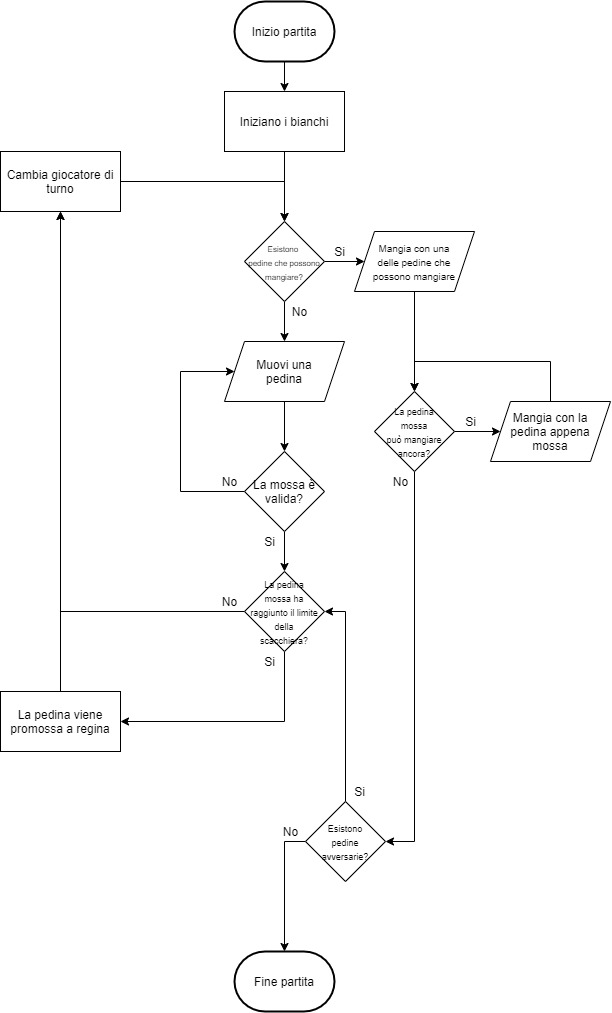
\includegraphics[scale=.5]{GameFlowChart}
\caption{Diagramma di flusso di una partita di dama usato come riferimento durante lo sviluppo}
\label{img:GameFC}
\end{figure}

\begin{itemize}
\item \textbf{14/08/2020}
	\begin{itemize}
	\item \textbf{Inizio Storia 6}
	\item Creazione dello script Server.cs
	\item All'interno dello script Server.cs definiamo la classe ServerClient per dare una definizione dei client che stabiliranno una connessione con il server
	\item Creazione del metodo Init di Server.cs dove inizializziamo le variabili del server come la lista dei client, settiamo un nuovo TcpListner che usa la socket 6321, avviamo il server e mettiamo il server in ascolto
	\item Creazione del metodo StartListening di Server.cs che chiama la funzione BeginAcceptTcpClient che svolge l'handshake per la connessione Tcp
	\item Creazione del metodo AcceptTcpClient di Server.cs per aggiungere alla lista clients l'oggetto ServerClient che verrà creato nel momento in cui un nuovo client si connetterà e rimettere subito dopo il server in ascolto
	\item Creazione del metodo IsConnected di Server.cs che controlla se un client è connesso al server
	\item Creazione del metodo Update di Server.cs dove richiamando il metodo IsConnected è possibile scoprire i client disconnessi, chiudere la connessione Tcp ed aggiungerli alla lista degli utenti disconnessi, oltre a creare un oggetto StreamReader che legga i messaggi inviati dai client ancora connessi. I client disconnessi verranno poi eliminati sia dalla lista disconnectList che dalla lista clients
	\item Creazione del metodo OnIncomingData di Server.cs per stabilire il protocollo che il server seguirà quando riceverà messaggi dai client (al momento lo definiremo solo con un log che stamperà a video il nome del client che ha inviato il messaggio ed il testo del messaggio ricevuto)
	\item Creazione del metodo Broadcast di Server.cs per inviare messaggi da parte del server alla lista di client connessi
	\item \textbf{Fine Storia 6}
	\end{itemize}
\item \textbf{17/08/2020}
	\begin{itemize}
	\item \textbf{Inizio Storia 7}
	\item Creazione dello script Client.cs
	\item All'interno dello script Client.cs definiamo la classe GameClient che sarà il tipo con cui identifichermo i client veri e propri
	\item Creazione del metodo ConnectToServer di Client.cs dove viene fatta richiesta di connessione al server alla socket 6321 e vengono inizializzati i reader e i writer
	\item Creazione del metodo OnIncomingData di Client.cs che definisce il protocollo che il client seguirà quando riceverà messaggi dal server (al momento lo definiremo solo con un log che stamperà a video il testo del messaggio ricevuto)
	\item Creazione del metodo Send di Client.cs per inviare messaggi al server
	\item Creazione del metodo Update di Client.cs che terrà il client in ascolto per eventuali messaggi da parte del server
	\item Creazione del metodo CloseSocket di Client.cs che terminerà la connessione chiudendo reader, writer e socket
	\item Creazione dei metodo OnApplicationQuit e OnDisable di Client.cs che chiama il metodo CloseSocket per terminare la connessione rispettivamente alla chiusura dell'applicazione e alla disattivazione dell'oggetto client
	\item \textbf{Fine Storia 7}
	\end{itemize}
\item \textbf{18/08/2020}
	\begin{itemize}
	\item \textbf{Inizio Storia 8}
	\item Creazione di una nuova scena in Unity che chiameremo Menu e utilizzeremo per l'appunto per il menù principale del gioco
	\item Creazione dello script GameManager.cs in cui viene codificato il funzionamento dei pulsanti sul menù.
	\item Creazione dei metodi Connect Button e HostButton di GameManager.cs che saranno i metodi che verranno chiamati nei metodi OnClick dei pulsanti Connettiti e Ospita
	\item Utilizzando l'editor di Unity, nella scena Menu creiamo i pulsanti e le interfacce grafiche del menù (pulsanti Connettiti e Ospita, schermata di inserimento dell'IP con pulsanti di conferma e per tornare indietro e schermata di attesa di connessione con pulsante per tornare indietro)
	\item Creazione del metodo ConnectToServerButton di GameManager.cs, che sarà il metodo che verrà chiamato nel metodo OnClick del pulsante Connettiti del sottomenù Connect, che per il momento resterà vuoto
	\item Creazione del metodo BackButton di GameManager.cs che sarà il metodo che verrà chiamato nel metodo OnClick dei pulsanti Indietro e Annulla rispettivamente del sottomenù Connect e Host
	\item \textbf{Fine Storia 8}
	\item \textbf{Release 0.6:} In questa release tardiva è stata aggiunta l'interfaccia del menù e la sua struttura base, oltre alle basilari funzionalità di navigazione all'interno del menù stesso
	\item \textbf{Inizio Storia 9}
	\item Nel metodo ConnectToServerButton di GameManager.cs inseriamo l'indirizzo Ip per la connessione di default come localhost, generiamo l'istanza di un oggetto Client e ne chiamiamo il metodo ConnectToServer
	\item Nel metodo HostButton di GameManager.cs codifichiamo la generazione di un'istanza di un oggetto Server e ne chiamiamo il metodo Init. Generiamo anche qui l'istanza di un oggetto Client e ne chiamiamo il metodo ConnectToServer specificando come indirizzo Ip il localhost
	\item Creiamo un inputField nel menù per l'inserimento del nome del client
	\item Modifichiamo lo script Client.cs per specificare un nome dell'oggetto Client, e modifichiamo anche i metodi ConnectToServerButton e HostButton di GameManager.cs per acquisire dall'input del menù il nome del client o per dare di default rispettivamente il nome Client e Host
	\item Bugfix per risolvere il problema che avviene nel momento in cui si crea un server ed un client, e si esce dalla schermata di attesa: in questo caso il server precedentemente creato non viene distrutto e rientrando nella schermata di attesa connessione ci ritroveremo con due istanze di un oggetto Server e di un oggetto Client. Aggiungiamo quindi il codice necessario per distruggere il server (se esiste) ed il client nel metodo BackButton di GameManager.cs
	\item \textbf{Fine Storia 9}
	\item \textbf{Release 0.7:} In questa release, dai log di debug è possibile notare che la connessione tra due giocatori funziona perfettamente seppure non sono ancora in grado di comunicare tra loro
	\end{itemize}
\item \textbf{19/08/2020}
	\begin{itemize}
	\item \textbf{Inizio Storia 10}
	\item Definiamo il nostro standard per i messaggi che verranno inviati tra client e server: la prima lettera indicherà il mittente, "S" (server) o "C" (client);
Il resto dei caratteri indicherà il tipo di messaggio, "WHO" (identificazione), "CNN" (connessione), "MOV" (mossa), "MSG" (messaggio chat);
Poi un carattere pipe ($|$) ricoprirà il ruolo di divisore tra i parametri passati nel messaggio Tcp in base alla sua natura (nome client + bool per identificare se il client è anche l'host nei messaggi di identificazione, nome client nei messaggi di connessione, posizione iniziale della pedina + posizione di arrivo della pedina nei messaggi di mossa, stringa contenente il messaggio di chat)
	\item Nello script Server.cs creiamo un override del metodo Broadcast che anziché prendere una stringa ed una lista di ServerClient come parametri in ingresso, prenderà un solo oggetto ServerClient anziché la lista. In questo metodo ci limiteremo a creare una nuova lista di ServerClient con un unico elemento che sarà il ServerClient che è stato passato in ingresso
	\item Modifichiamo il metodo AcceptTcpClient in Server.cs per inserire un Broadcast diretto agli altri client connessi al server per notificarli della connessione di un nuovo utente. Modifichiamo il metodo OnIncomingData in Client.cs per gestire il messaggio in questione inviato dal server
	\item Il metodo OnIncomingData sia in Server.cs che in Client.cs prenderà la stringa ricevuta attraverso la connessione Tcp e eseguirà uno Split in corrispondenza del carattere "$|$", per poi eseguire uno switch dove i vari casi dipenderanno dalla prima stringa. Quindi in questo caso ci curiamo del case "SWHO": per ogni client nella lista dei client connessi verrà chiamato il metodo UserConnected che istanzierà un oggetto GameClient e assegnerà il loro nome ad ognuno di essi. Infine il GameClient verrà aggiunto alla lista "players". Dopodiché verrà inviato dal client al server il messaggio "CWHO" che notificherà la volontà di connettersi
	\item Nello script Server.cs, nel metodo OnIncomingData, nel case "CWHO", il server prenderà i parametri del client che sta cercando di connettersi e dopodiché notificherà a tutti i client con un broadcast con un messaggio "SCNN" l'avvenuta connessione del nuovo client. Nel metodo OnIncomingData di Client.cs ogni client aggiungerà alla propria lista players il nuovo client (se la lista players raggiung ela dimensione 2 si inizia la partita)
	\item Bugfix: entrambi i giocatori una volta entrati in partita risultano come giocatore nero; risolviamo assegnando di default le pedine bianche all'host
	\item Modifichiamo il metodo EndTurn in CheckersBoard.cs per creare il messaggio "CMOV" che verrà inviato al server per notificare la mossa appena conclusa. Il messaggio conterrà le coordinate x ed y della posizione iniziale e della posizione finale della pedina. Nello script Server.cs, nel metodo OnIncomingData, nel case "CMOV", semplicemente, invieremo il medesimo messaggio in broadcast ai client connessi con la sigla "SMOV". Nello script Client.cs, nel metodo OnIncomingData, nel case "SMOV", chiamiamo il metodo TryMove dell'istanza CheckersBoard, passando le due coppie di coordinate x e y contenute nel messaggio
	\item Bugfix nel metodo CheckVictory di CheckersBoard.cs: il conteggio delle pedine rimanenti avveniva in un timing errato rispetto all'ultima pedina mangiata
	\item \textbf{Fine Storia 10}
	\item \textbf{Release 0.8:} Il gioco nella sua versione multiplayer è funzionante e senza bug. Sono ancora richieste delle migliorie, ma questa potremmo considerarla la prima release totalmente funzionale
	\end{itemize}
\item \textbf{20/08/2020}
	\begin{itemize}
	\item \textbf{Inizio Storia 11}
	\item Dopo aver acquistato il pacchetto base degli asset gratuiti di Unity, nella scena Game inseriamo l'elemento acqua sotto la scacchiera ed uno skybox notturno
	\item Copiamo il modello 3D della scacchiera insieme al resto della scena Game e li incolliamo nella scena Menu, eliminando lo script CheckersBoard.cs da questa versione dell'oggetto
	\item Inseriamo anche qualche pedina sull'oggetto 3D, dando loro un aspetto disordinato e piacevole da vedere. Regoliamo inoltre la posizione della camera sulla scena, cercando di dare una maggiore idea di dinamismo
	\item Creiamo le strutture grafiche che ci serviranno per implementare le notifiche durante la partita
	\item Nello script CheckersBoard.cs codifichiamo i metodi che ci permetteranno di gestire queste notifiche: Alert e UpdateAlert. Nel primo semplicemente verrà settato il testo della notifica, impostato il tempo in cui è stato avviato l'ultimo alert e settato un bool che indica la notifica come attiva. Nel secondo faremo in modo che dopo 1.5 secondi l'opacità della notifica inizi a calare e che dopo 2.5 secondi sia sparita del tutto
	\item Nel metodo Start di CheckersBoard.cs chiamiamo il metodo Alert in modo tale che ci notifichi il nome dei due giocatori della partita. Aggiungiamo le chiamate ad Alert anche nel metodo EndTurn, così che ogni volta che un giocatore passa il turno, ci sarà una notifica che ci avvertirà di chi è il turno attuale
	\item \textbf{Fine Storia 11}
	\item \textbf{Release 0.9:} Non ci sono stati molti cambiamenti funzionali dalla release precedente a questa, ma da un punto di vista grafico possiamo decisamente considerare questa nuova release molto più piacevole (anche se avevo iniziato a lavorarci non sono state implementate la telecamera mobile nella scena del menù e l'animazione "flip" della promozione a regina di una pedina in quanto non strettamente necessarie e per questo sono state depennate)
	\item \textbf{Inizio Storia 12}
	\item Creazione nuovo pulsante "Gioca in locale" nel menù di gioco per l'implementazione della partita in locale. Nello script GameManager.cs implementiamo il metodo LocalButton che verrà chiamato dal metodo OnClick del pulsante. In questo metodo verrà semplicemente cambiata la scena passando da Menu a Game
	\item Nello script CheckersBoard.cs modifichiamo vari metodi per permettere la partita in locale, utilizzando come discriminatore (o come valore booleano negli if) l'esistenza o meno di un client
	\item Diverse iterazioni fa avevo commentato una parte di codice che serviva per testare il funzionamento del gioco cambiando il turno del giocatore che muoveva. Ora questo frammento di codice verrà utilizzato per far funzionare la partita locale
	\item Aggiungiamo il caso dell'alert in assenza di client: in questo caso l'alert ci avvertirà solo del colore di pedine che deve muovere.
	\item \textbf{Fine Storia 12}
	\item \textbf{Release 0.10:} L'unico cambiamento di questa release rispetto alla precedente è la possibiltà di giocare anche in locale. Originariamente non era considerato un requisito funzionale, ma essendo di facile implementazione è stato aggiunto
	\end{itemize}
\item \textbf{21/08/2020}
	\begin{itemize}
	\item \textbf{Inizio Storia 13}
	\item Creiamo un generico oggetto 3D quadrato 1mx1m (le dimensioni di una tessera della scacchiera) e nel metodo Start di CheckersBoard.cs lo posizioniamo 100m sotto la scacchiera
	\item Creiamo il metodo Highlight in CheckersBoard.cs che servirà per posizionare l'oggetto precedentemente creato sotto una pedina e chiamiamo questo metodo alla fine di ScanForcedMoves
	\item Bugfix dovuto al mancato spawn dell'oggetto 3D. Inseriamo una chiamata a ScanForcedMoves alla fine di EndTurn
	\item Bugfix dovuto ad uno strano posizionamento dell'oggetto 3D dopo una mossa non valida. Inseriamo una chiamata ad Highlight prima di ogni return in TryMove
	\item Animiamo gli oggetti 3D dando loro una rotazione all'interno del metodo Update in CheckersBoard.cs
	\item All'oggetto 3D colleghiamo un effetto particellare per renderlo maggiormente visibile: dopo un lungo processo di trial and error è stato raggiunto un risultato soddisfacente con dei raggi di luce che si diffondono in maniera radiale sopra l'oggetto 3D, che alla fine decido di rendere invisibile, lasciando visibile solo la luce per gusti estetici
	\item Copio l'oggetto 3D 1 volta poiché nella dama è impossibile avere più di due pedoni che possono mangiare contemporaneamente e modifico il codice per agire su entrambi gli oggetti
	\item \textbf{Fine Storia 13}
	\item \textbf{Release 0.11:} Questa aggiunta estetica rende il gioco sicuramente migliore, mettendo così in risalto una regola che potrebbe sfuggire alla vista di giocatori meno esperti, risultando così una feature sia estetica che funzionale
	\end{itemize}
\item \textbf{22/08/2020}
	\begin{itemize}
	\item \textbf{Inizio Storia 14}
	\item Creiamo il case "CMSG" nello switch nel metodo OnIncomingData di Server.cs per poter gestire i messaggi della chat che andremo ad implementare: molto semplicemente il messaggio ricevuto verrà mandato in broadcast ai client connessi con la sigla iniziale "SMSG" e il nome del client che l'ha inviato
	\item Creiamo il case "SMSG" nello switch nel metodo OnIncomingData di Client.cs per poter gestire i messaggi della chat ricevuti dal server. Chiamiamo il metodo ChatMessage dall'istanza di CheckersBoard, passando il testo del messaggio.
	\item Creiamo gli elementi grafici che comporranno la chat nella schermata in-game: un pannello dove verranno aggiunti i messaggi inviati e ricevuti, uno spazio di input dove inserire il messaggio da inviare e il punlsante per confermare l'invio del messaggio
	\item Creazione metodo ChatMessage e SendMessage di CheckersBoard.cs rispettivamente per stampare a video sul pannello della chat ed inviare i messaggi scritti sullo spazio di input
	\item Modifichiamo il metodo Start di CheckersBoard.cs per creare un'istanza della chat nella partita online ma non nella partita in locale
	\item \textbf{Fine Storia 14}
	\item \textbf{Release 0.12:} Questa release aggiunge una chat in-game perfettamente funzionante che permette di comunicare tra i due giocatori. A livello funzionale il progetto è completo. Mancano solo alcune migliorie grafiche
	\end{itemize}
\item \textbf{Fine - 24/08/2020}
	\begin{itemize}
	\item \textbf{Inizio Storia 15}
	\item Nella scelta di migliorare graficamente il progetto decidiamo uno stile semplice ma di impatto, usando come font predominante un font pixelato gratuitamente acquisito sullo Unity asset store e come colori le scritte bianche su sfondo nero
	\item Creiamo una scritta che graficamente faccia da titolo per l'applicazione. Usiamo i tool grafici direttamente messi a disposizione da Unity, senza servirci di programmi di grafica esterni
	\item Modifichiamo tutte le interfacce grafiche del software secondo lo standard scelto
	\item Creiamo un'animazione per il mouseover dei pulsanti del menù principale
	\item Modifichiamo il metodo Victory in CheckersBoard.cs , inserendo una chiamata al metodo Alert che ci notifichi quale giocatore ha vinto. Inoltre modifichiamo il metodo Update in CheckersBoard.cs per chiudere la partita, distruggendo le istanze di Server e Client e tornare al menù principale dopo 3 sec
	\item \textbf{Fine Storia 15} 
	\item \textbf{Release 1.0:} Questa ultima release la possiamo considerare completa e priva di bug e pronta per essere consegnata al cliente entro il tempo limite che ci siamo fissati. i requisiti funzionali sono stati implementati tutti correttamente ed il prodotto è visivamente piacevole
	\end{itemize}
\end{itemize}

Dopo aver discusso col cliente e aver preso in carico le modifiche concordate, ricomincia il processo di sviluppo:

\begin{figure}[H]
\centering
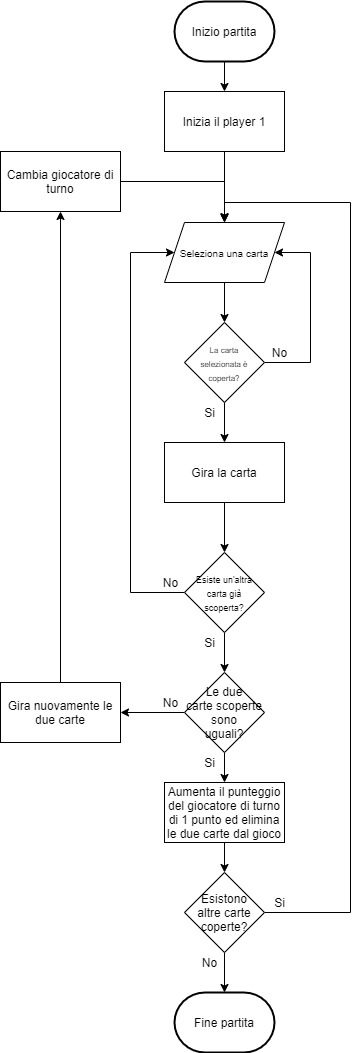
\includegraphics[scale=.5]{MemoryFlowChart}
\caption{Diagramma di flusso di una partita di memory usato come riferimento durante lo sviluppo}
\label{img:MemoryFC}
\end{figure}

\begin{itemize}
\item \textbf{Inizio - 31/08/2020}
	\begin{itemize}
	\item \textbf{Inizio Storia 1}
	\item Creazione del modello 3D del tavolo da gioco e delle carte. Si è scelto uno stile grafico affine a quello del gioco della Dama già implementato
	\item Creazione dello script MemoryTable.cs: conterrà la maggior parte del codice riguardante il gioco. Qui verranno implementati i metodi che regoleranno il funzionamento della partita
	\item Creazione dello script Card.cs usato per definire la classe Card che rappresenta le carte del gioco e ne contiene gli attributi ed i metodi
	\item Creazione dei metodi GenerateDeck, GenerateCard, GenerateCopy, ShuffleDeck e PositionCards di MemoryTable.cs: il primo chiamerà gli altri 4 rispettivamente per creare le prime 20 carte di cui è composto il mazzo, creare le restanti 40 carte copie delle prime 20, mescolare il mazzo (usando dei numeri randomici per ogni carta, che detteranno di quante posizioni verrà spostata la suddetta carta) e posizionare le carte del mazzo coperte sul tavolo da gioco
	\item \textbf{Fine Storia 1}
	\item \textbf{Inizio Storia 2}
	\item Creazione del metodo CardClicker di MemoryTable.cs che viene chiamato nel metodo Update per controllare se l'utente cliccando con il tasto sinistro del mouse clicchi o meno una carta
	\item Creazione del metodo FlipCard di MemoryTable.cs che viene chiamato da CardClicker se si clicka effettivamente su una carta: questo metodo fa girare una carta al gioctore di turno se essa non è già girata e se è la prima ad essere stata girata durante il turno, gli permette di girarne un'altra, salvando il valore di quella appena girata. Se invece quando viene girata la carta ne esiste una già girata, verrà chiamato il metodo IsAMatch di Card.cs. Se le due carte sono una coppia verrà incrementato il punteggio a video del giocatore di turno, cancellato il riferimento alla carta girata in precedenza, diminuito il numero di coppie di carte ancora in gioco e se questo numero arriva a 0 si conclude il gioco. Se invece le due carte non sono una coppia, verrà settato un timer che dopo 1.5 secondi, chiamerà il metodo ReFlip di MemoryTable.cs, che rimetterà le carte in posizione coperta e infine verrà cambiato il giocatore di turno
	\item Creazione del metodo IsAMatch di Card.cs per verificare se le due carte (quella dalla cui istanza viene chiamato il metodo e quella che viene passa come parametro) sono uguali sia nel seme che nel valore di carta. Se lo sono il metodo restituirà un valore booleano vero, altrimenti, oltre a restituire falso, resetterà i valori delle due carte e ne cancellerà i riferimenti salvati
	\item Creazione del metodo EndGame di MemoryTable.cs che viene chiamato nel momento in cui non ci sono più coppie coperte in gioco. Semplicemente in questo metodo se il punteggio del primo giocatore è superiore a quello del secondo faremo apparire una notifica che ci avvertirà della vittoria del primo giocatore; in caso opposto ci notificherà della vittoria del secondo; nel caso in cui i due punteggi si eguaglino verrà comunicato il pareggio. Dopo 2 secondi si tornerà al menù del memory
	\item \textbf{Fine Storia 2}
	\item \textbf{Release 1.1:} In questa release inseriamo il gioco del Memory completo e perfettamente funzionante, anche se mancano ancora delle accortezze per quanto riguarda l'interfaccia
	\end{itemize}
\item \textbf{Fine - 31/08/2020}
\item \textbf{Inizio - 01/09/2020}
	\begin{itemize}
	\item \textbf{Inizio Storia 3}
	\item Nell'editor di Unity creiamo 4 pannelli con testo: due che indicano il punteggio dei due giocatori, uno che indica il numero di coppie rimaste e uno, invisibile di default che useremo per notificare la fine della partita
	\item Creazione del metodo UpdateScore di MemoryTable.cs che viene chiamato quando uno dei due giocatori segna un punto. Questo metodo modifica il testo dei 3 pannelli testuali su schermo, aggiornando ad ogni chiamata i 3 valori (il punteggio del primo giocatore, il punteggio del secondo giocatore e il numero di coppie rimanenti).
	\item \textbf{Fine Storia 3}
	\item \textbf{Release 1.2:} Questa release non apporta modifiche di tipo logico o funzionale al gioco, ma lo rende più userfriendly mostrando a video i punteggi dei giocatori e le coppie di carte rimaste, rendendolo più simile ad un gioco
	\item \textbf{Inizio Storia 4}
	\item Creazione delle scene MemoryMenu e MainMenu dall'editor di Unity. Nella prima inseriamo un pulsante che permette di iniziare una partita a memory ed uno che permette di cambiare scena e tornare al menù principale. Nel secondo inseriamo due pulsanti che permettano di navigare da questo menù ai menù di Dama o Memory
	\item Creazione degli script GameMenagerMemo.cs e GameManagerMain.cs dove sono stati codificati i funzionamenti dei pulsanti rispettivamente del menù di Memory e del menù principale
	\item Modifica della scena Menu e dello script GameManager.cs, per inserire un nuovo pulsante che permetta di tornare al menù principale dal menù della Dama
	\item \textbf{Fine Storia 4}
	\item \textbf{Inizio Storia 5}
	\item Modifica delle scene MemoryMenu e MainMenu, dove andremo ad applicare lo stesso standard estetico del menù di Dama, inseriamo inoltre lo skybox e l'effetto acqua sulle nuove scene (Memory, MemoryMenu, MainMenu) e i modelli 3D dei giochi privati di script ed inseriti per scopi estetici
	\item \textbf{Fine Storia 5}
	\item \textbf{Release 1.3:} Questa release inserisce perfettamente un menù principale e lo imposta come prima scena del videogioco, permette la navigazione tra i vari menù e permette sia di giocare al memory che alla dama nella stessa sessione del software. Il progetto allo stato attuale è pronto per la sua pubblicazione ed è in uno stato tale in cui sarebbe possibile implementare ulteriori giochi senza troppo lavoro
	\end{itemize}
\item \textbf{Fine - 01/09/2020}
\end{itemize}

\subsection{Class Diagram}
Il diagramma delle classi (class diagram) serve a fornire una vista strutturale del sistema in termini di attributi e metodi delle classi e le relazioni che intercorrono tra loro. Il diagramma fa riferimento alle classi effettivamente realizzate e alle strutture dati effettivamente impiegate, infatti non lo definiamo uno schema concettuale, ma implementativo.

Nelle classi gli attributi sono scritti nella forma:\newline
\textbf{\textit{NomeAttributo : TipoAttributo = ValoreDefault}}

E i metodi nella forma:\newline
\textbf{\textit{NomeMetodo(ListaTipoParametri) : TipoValoreRestituito}}

\begin{figure}[H]
\centering
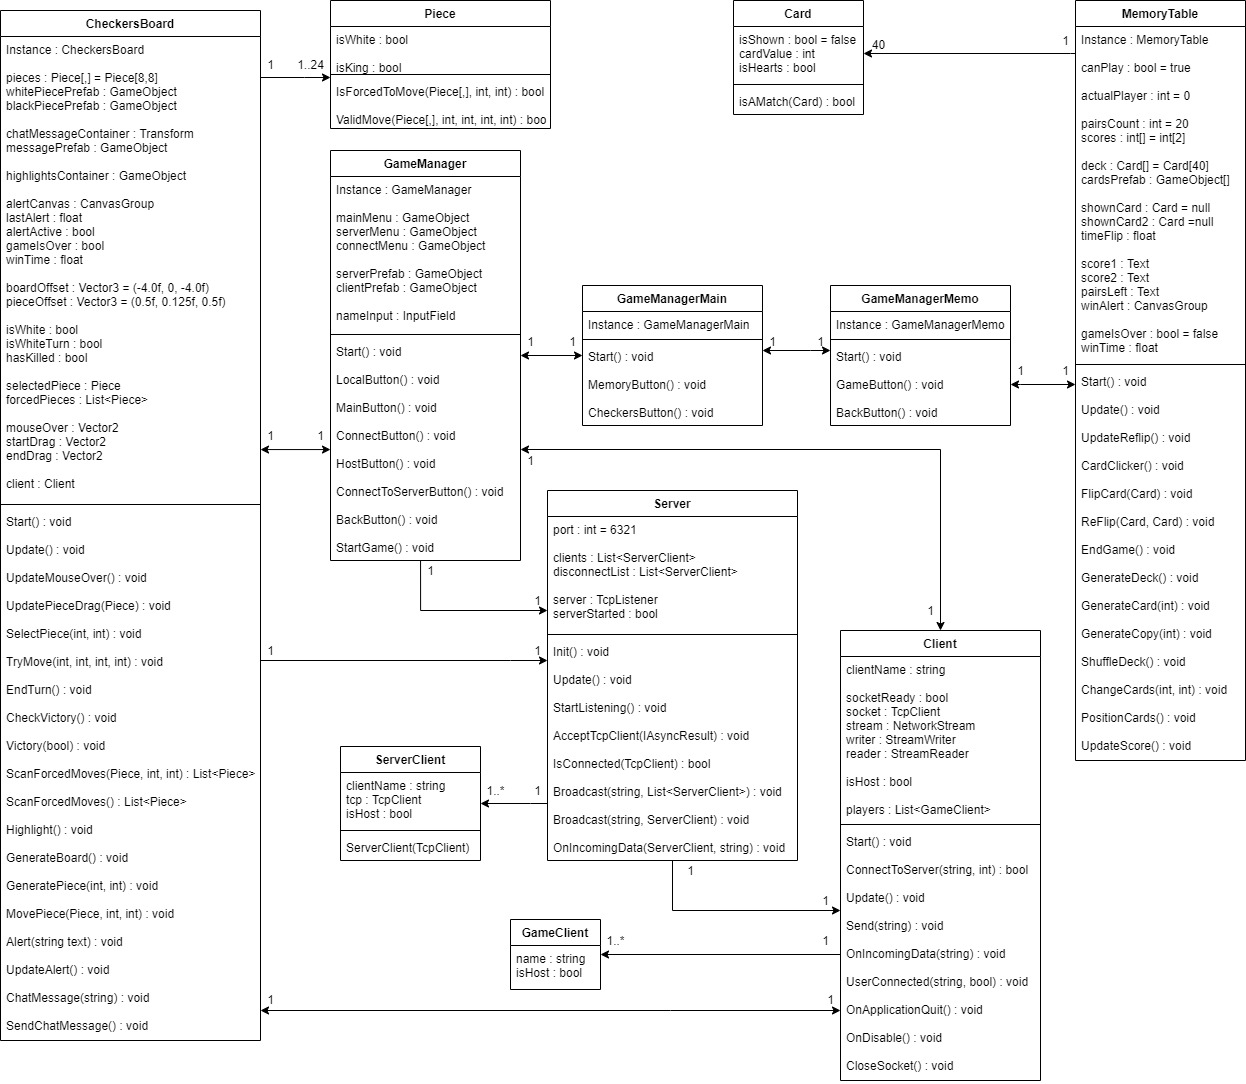
\includegraphics[scale=.30]{ClassDiagram}
\caption{Diagramma delle classi del sistema}
\label{img:classdiagram}
\end{figure}

Nella figura \ref{img:classdiagram} possiamo vedere il diagramma delle classi sviluppato a seguito della conclusione del progetto per dare una rappresentazione completa delle classi e delle loro relazioni. Come è possibile notare non esistono classi frutto di aggregazioni, questo perché sia nel caso delle pedine della dama che delle carte del memory, non mi era sembrato conveniente, a livello di sfruttamento delle risorse, creare una ipotetica superclasse di pezzi che avrei chiamato Team o una superclasse di carte che avrei chiamato Deck. Invece le classi Piece e Card vengono utilizzate per definire le istanze di oggetti fondamentali all'interno di CheckersBoard e MemoryTable, ovvero Pieces e Deck (definiti come array di oggetti di classe rispettivamente Piece e Card). Infatti le loro occorrenze all'interno dei due script sono numeri precisi: 24 (12 pedine bianche e 12 pedine nere) occorrenze di Piece dentro CheckersBoard e 40 (10 carte per seme ripetute due volte) occorrenze di Card dentro MemoryTable; va fatto notare inoltre che le occorrenze di Piece sono comprese tra 1 e 24 poiché esse possono variare nel tempo, visto che nel momento in cui una pedina viene mangiata durante una partita, la sua istanza come GameObject viene distrutta, però in nessun caso le pedine potranno essere di numero inferiore ad 1, quindi durante il ciclo di vita di un'istanza di CheckersBoard, il numero di istanze di Piece può diminuire fino ad un minimo di 1.

Salta inoltre subito all'occhio che in nessuna relazione è mai presente più di una occorrenza di CheckersBoard o di MemoryTable: questo perché in nessun caso esisterà contemporaneamente più di una istanza delle due classi.

La classe MemoryTable è legata solo da un'altra relazione con GameManagerMemo, in quanto esse richiamano il costruttore dell'altra classe nel momento in cui distruggono la propria istanza. Medesimo discorso vale per la relazione tra CheckersBoard e GameManager.

Sia GameManager che GameManagerMemo sono a loro volta in relazione con GameManagerMain, in quanto anche in questo caso esse chiamano vicendevolmente il costruttore dell'altra classe nel momento in cui vengono distrutte.

GameManager presenta poi una relazione con Server e Client, in quanto è lei stessa a chiamare dentro di se i metodi Init di Server e Start di Client.

Server a sua volta presenta una relazione con CheckersBoard, poiché sarà la stessa CheckersBoard, che prima di distruggere la propria istanza, distruggerà l'istanza di Server (così come quella di Client). Inoltre, la classe server è in relazione uno a molti con ServerClient, la classe che definisce l'oggetto che rappresenta i client connessi al server, oltre che con Client ovviamente, dal momento che essa è la classe con cui interagisce maggiormente tramite il metodo Broadcast e OnIncomingData.

Allo stesso modo Client, oltre che con Server, GameManager e CheckersBoard è in relazione con la classe GameClient, la classe definita per descrivere gli oggetti che rappresentano le istanze degli altri client connessi al server.

\section{Conclusioni e codice}
Il progetto è stato completato nei tempi previsti ed entro la data di consegna prefissata. La documentazione qui prodotta presenta un'analisi metodologica ed una descrizione del lavoro svolto abbastanza miticolosa, cercando di mantenere un linguaggio che per lo più risulti comprensibile anche ad un ipotetico cliente, o generico lettore, sprovvisto di competenze in ambito informatico. Il software risulta funzionante e privo di bug ed è stato testato per questo tipo di indagine più volte.

Possiamo quindi in conclusione affermare che lo sviluppo del progetto si è concluso con risultato positivo.

Qui di seguito verrà mostrato il codice sviluppato per il progetto, reperibile anche all'indirizzo: \url{https://github.com/MTheHead61/SoftwareEngProject}.

\begin{lstlisting}[language={[Sharp]C}, caption={CheckersBoard.cs}, label={CheckersBoardScript}]
using System.Collections.Generic;
using System.Collections;
using UnityEngine;
using UnityEngine.UI;
using UnityEngine.SceneManagement;

public class CheckersBoard : MonoBehaviour
{
	public static CheckersBoard Instance { set; get; }
	
	public Piece[,] pieces = new Piece[8,8];
	public GameObject whitePiecePrefab;
	public GameObject blackPiecePrefab;
	
	public Transform chatMessageContainer;
	public GameObject messagePrefab;
	
	public GameObject highlightsContainer;

	public CanvasGroup alertCanvas;
	private float lastAlert;
	private bool alertActive;
	private bool gameIsOver;
	private float winTime;

	private Vector3 boardOffset = new Vector3(-4.0f, 0, -4.0f);
	private Vector3 pieceOffset = new Vector3(0.5f, 0.125f, 0.5f);

	public bool isWhite;
	private bool isWhiteTurn;
	private bool hasKilled;

	private Piece selectedPiece;
	private List<Piece> forcedPieces;

	private Vector2 mouseOver;
	private Vector2 startDrag;
	private Vector2 endDrag;
	
	private Client client;

	private void Start()
	{	
		Instance = this;
		
		client = FindObjectOfType<Client>();
		
		foreach(Transform t in highlightsContainer.transform)
		{
			t.position = Vector3.down * 100;
		}
		
		if(client)
		{
			isWhite = client.isHost;
			Alert(client.players[0].name + " VS " + client.players[1].name);
		}
		else
		{
			Alert("Turno giocatore bianco");
			Transform c = GameObject.Find("Canvas").transform;
			foreach(Transform t in c)
			{
				t.gameObject.SetActive(false);
			}
			c.GetChild(0).gameObject.SetActive(true);
		}
		
		isWhiteTurn = true;
		forcedPieces = new List<Piece>();
		GenerateBoard();
	}

	private void Update()
    {
		if(gameIsOver)
		{
			if(Time.time - winTime > 3.0f)
			{
				Server server = FindObjectOfType<Server>();
				Client client = FindObjectOfType<Client>();
				
				if(server)
					Destroy(server.gameObject);
			
				if(client)
					Destroy(client.gameObject);
				
				SceneManager.LoadScene("Menu");
			}
			return;
		}
		foreach(Transform t in highlightsContainer.transform)
		{
			t.Rotate(Vector3.up * 90 * Time.deltaTime);
		}
		
		UpdateAlert();
		UpdateMouseOver();

        if((isWhite)?isWhiteTurn:!isWhiteTurn)
        {
			int x = (int)mouseOver.x;
			int y = (int)mouseOver.y;

			if (selectedPiece != null)
				UpdatePieceDrag(selectedPiece);

			if (Input.GetMouseButtonDown(0))
				SelectPiece(x, y);

			if (Input.GetMouseButtonUp(0))
				TryMove((int)startDrag.x, (int)startDrag.y, x, y);
		}

	}
	
	private void UpdateMouseOver()
    {
		if(!Camera.main)
        {
			Debug.Log("Camera main non trovata");
			return;
        }
		RaycastHit hit;
		if(Physics.Raycast(Camera.main.ScreenPointToRay(Input.mousePosition),out hit, 25.0f, LayerMask.GetMask("Board")))
        {
			mouseOver.x = (int)(hit.point.x - boardOffset.x);
			mouseOver.y = (int)(hit.point.z - boardOffset.z);
        }
		else
        {
			mouseOver.x = -1;
			mouseOver.y = -1;
        }
    }
	
	private void UpdatePieceDrag(Piece p)
    {
		if (!Camera.main)
		{
			Debug.Log("Camera main non trovata");
			return;
		}
		RaycastHit hit;
		if (Physics.Raycast(Camera.main.ScreenPointToRay(Input.mousePosition), out hit, 25.0f, LayerMask.GetMask("Board")))
		{
			p.transform.position = hit.point + Vector3.up;

		}
	}

	private void SelectPiece(int x, int y)
    {
		if (x < 0 || x >= 8 || y < 0 || y >= 8)
			return;

		Piece p = pieces[x, y];
		if(p != null && p.isWhite == isWhite)
        {
			if (forcedPieces.Count == 0)
			{
				selectedPiece = p;
				startDrag = mouseOver;
			}
            else
            {
				if (forcedPieces.Find(fp => fp == p) == null)
					return;

				selectedPiece = p;
				startDrag = mouseOver;
            }
        }
    }
	
	public void TryMove(int x1, int y1, int x2, int y2)
    {
		forcedPieces = ScanForcedMoves();

		//Multiplayer
		startDrag = new Vector2(x1, y1);
		endDrag = new Vector2(x2, y2);
		selectedPiece = pieces[x1, y1];

		//Fuori limite
		if (x2 < 0 || x2 >= 8 || y2 < 0 || y2 >= 8)
        {
			if (selectedPiece != null)
				MovePiece(selectedPiece, x1, y1);

			startDrag = Vector2.zero;
			selectedPiece = null;
			Highlight();
			return;
        }

		if (selectedPiece != null)
        {
			//Nessuna mossa
			if (endDrag == startDrag)
            {
				MovePiece(selectedPiece, x1, y1);
				startDrag = Vector2.zero;
				selectedPiece = null;
				Highlight();
				return;
			}

            //Controllo mossa valida
            if (selectedPiece.ValidMove(pieces, x1, y1, x2, y2))
            {
                //Mangiato
                if (Mathf.Abs(x2 - x1) == 2)
                {
					Piece p = pieces[(x1 + x2) / 2, (y1 + y2) / 2];
                    if (p != null)
                    {
						pieces[(x1 + x2) / 2, (y1 + y2) / 2] = null;
						DestroyImmediate(p.gameObject);
						hasKilled = true;
					}
				}

                if (forcedPieces.Count != 0 && !hasKilled)
                {
					MovePiece(selectedPiece, x1, y1);
					startDrag = Vector2.zero;
					selectedPiece = null;
					Highlight();
					return;
				}

				pieces[x2, y2] = selectedPiece;
				pieces[x1, y1] = null;
				MovePiece(selectedPiece, x2, y2);

				EndTurn();
            }
            else
            {
				MovePiece(selectedPiece, x1, y1);
				startDrag = Vector2.zero;
				selectedPiece = null;
				Highlight();
				return;
			}
        }

    }

	private void EndTurn()
    {
		int x = (int)endDrag.x;
		int y = (int)endDrag.y;
		
		//Promozione
        if (selectedPiece != null)
        {
            if (selectedPiece.isWhite && !selectedPiece.isKing && y == 7)
            {
				selectedPiece.isKing = true;
				selectedPiece.transform.Rotate(Vector3.right * 180);
            }
			else if (!selectedPiece.isWhite && !selectedPiece.isKing && y == 0)
			{
				selectedPiece.isKing = true;
				selectedPiece.transform.Rotate(Vector3.right * 180);
			}
		}
		
		if(client)
		{
			string msg = "CMOV|";
			msg += startDrag.x.ToString() + "|";
			msg += startDrag.y.ToString() + "|";
			msg += endDrag.x.ToString() + "|";
			msg += endDrag.y.ToString();
		
		client.Send(msg);
		}

		selectedPiece = null;
		startDrag = Vector2.zero;

		if (ScanForcedMoves(selectedPiece, x, y).Count != 0 && hasKilled)
			return;

		isWhiteTurn = !isWhiteTurn;
		hasKilled = false;
		CheckVictory();
		
		if(!gameIsOver)
		{
			if(!client)
			{
				isWhite = !isWhite;
				if(isWhite)
					Alert("Turno giocatore bianco");
				else
					Alert("Turno giocatore nero");
			}
			else
			{
				if(isWhite)
					Alert("Turno di " + client.players[0].name);
				else
					Alert("Turno di " + client.players[1].name);
			}
		}
		
		ScanForcedMoves();
    }

	private void CheckVictory()
    {
		var ps = FindObjectsOfType<Piece>();
		bool hasWhite = false, hasBlack = false;
		for (int i=0; i < ps.Length; i++)
        {
			if (ps[i].isWhite)
				hasWhite = true;
			else
				hasBlack = true;
        }

		if (!hasWhite)
			Victory(false);
		if (!hasBlack)
			Victory(true);
    }

	private void Victory(bool isWhite)
    {
		winTime = Time.time;
		
		if(isWhite)
			Alert("Il bianco vince!");
		else
			Alert("Il nero vince!");
		
		gameIsOver = true;
	}

	private List<Piece> ScanForcedMoves(Piece p, int x, int y)
    {
		forcedPieces = new List<Piece>();

		if (pieces[x, y].IsForcedToMove(pieces, x, y))
			forcedPieces.Add(pieces[x, y]);

		Highlight();
		return forcedPieces;
	}

	private List<Piece> ScanForcedMoves()
    {
		forcedPieces = new List<Piece>();

		for (int i = 0; i < 8; i++)
			for (int j = 0; j < 8; j++)
				if (pieces[i, j] != null && pieces[i, j].isWhite == isWhiteTurn)
					if (pieces[i, j].IsForcedToMove(pieces, i, j))
						forcedPieces.Add(pieces[i, j]);
		Highlight();
		return forcedPieces;
    }
	
	private void Highlight()
	{
		foreach(Transform t in highlightsContainer.transform)
		{
			t.position = Vector3.down * 100;
		}
		
		if (forcedPieces.Count > 0)
		{
			highlightsContainer.transform.GetChild(0).transform.position = forcedPieces[0].transform.position + Vector3.down * 0.1f;
			if (forcedPieces.Count > 1)
				highlightsContainer.transform.GetChild(1).transform.position = forcedPieces[1].transform.position + Vector3.down * 0.1f;
		}
	}

	private void GenerateBoard()
	{
		//Genera pezzi bianchi
		for (int y = 0; y < 3; y++)
		{
			bool oddRow = (y % 2 == 0);
			for(int x = 0; x < 8; x += 2)
			{
				GeneratePiece((oddRow) ? x : x + 1, y);
			}
		}

		//Genera pezzi neri
		for (int y = 7; y > 4; y--)
		{
			bool oddRow = (y % 2 == 0);
			for (int x = 0; x < 8; x += 2)
			{
				GeneratePiece((oddRow) ? x : x + 1, y);
			}
		}
	}
	
	private void GeneratePiece(int x, int y)
	{
		bool isPieceWhite = (y > 3) ? false : true;
		GameObject go = Instantiate((isPieceWhite) ? whitePiecePrefab : blackPiecePrefab) as GameObject;
		go.transform.SetParent(transform);
		Piece p = go.GetComponent<Piece>();
		pieces[x,y] = p;
		MovePiece(p, x, y);

	}
	
	private void MovePiece(Piece p, int x, int y)
    {
		p.transform.position = (Vector3.right * x) + (Vector3.forward * y) + boardOffset + pieceOffset;
    }

	public void Alert(string text)
	{
		alertCanvas.GetComponentInChildren<Text>().text = text;
		alertCanvas.alpha = 1;
		lastAlert = Time.time;
		alertActive = true;
	}

	public void UpdateAlert()
	{
		if(alertActive)
		{
			if(Time.time - lastAlert > 1.5f)
			{
				
				alertCanvas.alpha = 1 - ((Time.time - lastAlert) - 1.5f);
				
				if(Time.time - lastAlert > 2.5f)
				{
					alertActive = false;
				}
			}
		}
	}

	public void ChatMessage(string msg)
	{
		GameObject go = Instantiate(messagePrefab) as GameObject;
		go.transform.SetParent(chatMessageContainer);
		
		go.GetComponentInChildren<Text>().text = msg;
	}
	
	public void SendChatMessage()
	{
		InputField i = GameObject.Find("MessageInput").GetComponent<InputField>();
		
		if(i.text == "")
			return;
		
		client.Send("CMSG|" + i.text);
		
		i.text = "";
	}
}
\end{lstlisting}

\begin{lstlisting}[language={[Sharp]C}, caption={Piece.cs}, label={PieceScript}]
using System.Collections;
using UnityEngine;

public class Piece : MonoBehaviour
{
    public bool isWhite;
    public bool isKing;

    public bool IsForcedToMove(Piece[,] board, int x, int y)
    {
        if (isWhite||isKing)
        {
            if (x >= 2 && y <= 5)
            {
                Piece p = board[x - 1, y + 1];
                if (p != null && p.isWhite != isWhite)
                {
                    if (board[x - 2, y + 2] == null)
                        return true;
                }
            }

            if (x <= 5 && y <= 5)
            {
                Piece p = board[x + 1, y + 1];
                if (p != null && p.isWhite != isWhite)
                {
                    if (board[x + 2, y + 2] == null)
                        return true;
                }
            }
        }
        if (!isWhite||isKing)
        {
            if (x >= 2 && y >= 2)
            {
                Piece p = board[x - 1, y - 1];
                if (p != null && p.isWhite != isWhite)
                {
                    if (board[x - 2, y - 2] == null)
                        return true;
                }
            }

            if (x <= 5 && y >= 2)
            {
                Piece p = board[x + 1, y - 1];
                if (p != null && p.isWhite != isWhite)
                {
                    if (board[x + 2, y - 2] == null)
                        return true;
                }
            }
        }
        return false;
    }

    public bool ValidMove(Piece[,] board, int x1, int y1, int x2, int y2)
    {
        //Muoversi su un'altra pedina
        if (board[x2, y2] != null)
            return false;

        int deltaMove = Mathf.Abs(x1 - x2);
        int deltaMoveY = y2 - y1;

        if (isWhite || isKing)
        {
            if (deltaMove == 1)
            {
                if (deltaMoveY == 1)
                    return true;
            }
            else if (deltaMove == 2)
            {
                if (deltaMoveY == 2)
                {
                    Piece p = board[(x1 + x2) / 2, (y1 + y2) / 2];
                    if (p != null && p.isWhite != isWhite)
                        return true;
                }
            }
        }

        if (!isWhite || isKing)
        {
            if (deltaMove == 1)
            {
                if (deltaMoveY == -1)
                    return true;
            }
            else if (deltaMove == 2)
            {
                if (deltaMoveY == -2)
                {
                    Piece p = board[(x1 + x2) / 2, (y1 + y2) / 2];
                    if (p != null && p.isWhite != isWhite)
                        return true;
                }
            }
        }

        return false;
    
    }
}
\end{lstlisting}

\begin{lstlisting}[language={[Sharp]C}, caption={Server.cs}, label={ServerScript}]
using System.Collections;
using UnityEngine;
using System.Net.Sockets;
using System;
using System.Collections.Generic;
using System.Net;
using System.IO;

public class Server : MonoBehaviour
{
    public int port = 6321;

    private List<ServerClient> clients;
    private List<ServerClient> disconnectList;

    private TcpListener server;
    private bool serverStarted;

    public void Init()
    {
        DontDestroyOnLoad(gameObject);
		clients = new List<ServerClient>();
		disconnectList = new List<ServerClient>();
		
		try
		{
			server = new TcpListener(IPAddress.Any, port);
			server.Start();
			
			StartListening();
			serverStarted = true;
		}
		catch(Exception e)
		{
			Debug.Log("Socket errore: " + e.Message);
		}
    }
	
	private void Update()
	{
		if(!serverStarted)
			return;
		
		foreach(ServerClient c in clients)
		{
			//Client ancora connesso?
			if(!IsConnected(c.tcp))
			{
				c.tcp.Close();
				disconnectList.Add(c);
				continue;
			}
			else
			{
				NetworkStream s = c.tcp.GetStream();
				if(s.DataAvailable)
				{
					StreamReader reader = new StreamReader(s, true);
					string data = reader.ReadLine();
					
					if(data != null)
						OnIncomingData(c, data);
				}					
			}
		}
		for(int i = 0; i < disconnectList.Count - 1; i++)
		{
			//Avviso di disconnessione
			clients.Remove(disconnectList[i]);
			disconnectList.RemoveAt(i);
		}
	}
	
	private void StartListening()
	{
		server.BeginAcceptTcpClient(AcceptTcpClient, server);
	}
	
	private void AcceptTcpClient(IAsyncResult ar)
	{
		TcpListener listener = (TcpListener)ar.AsyncState;
		
		string allUsers = "";
		foreach(ServerClient i in clients)
		{
			allUsers += i.clientName + "|" ;
		}
		
		ServerClient sc = new ServerClient(listener.EndAcceptTcpClient(ar));
		clients.Add(sc);
		
		StartListening();
		
		Broadcast("SWHO|" + allUsers ,clients[clients.Count-1]);
	}
	
	private bool IsConnected(TcpClient c)
	{
		try
		{
			if(c != null && c.Client != null && c.Client.Connected)
			{
				if(c.Client.Poll(0,SelectMode.SelectRead))
					return !(c.Client.Receive(new byte[1], SocketFlags.Peek) == 0);
				
				return true;
			}
			else
				return false;
		}
		catch
		{
			return false;
		}
	}
	//Invio
	private void Broadcast(string data, List<ServerClient> cl)
	{
		foreach(ServerClient sc in cl)
		{
			try
			{
				StreamWriter writer = new StreamWriter(sc.tcp.GetStream());
				writer.WriteLine(data);
				writer.Flush();
			}
			catch(Exception e)
			{
				Debug.Log("Error: " + e.Message);
			}
		}
	}
	
	private void Broadcast(string data, ServerClient c)
	{
		List<ServerClient> sc = new List<ServerClient> { c };
		Broadcast(data, sc);
	}
	
	//Lettura
	private void OnIncomingData(ServerClient c, string data)
	{
		string[] aData = data.Split('|');
		
		switch(aData[0])
		{
			case "CWHO":
				c.clientName = aData[1];
				c.isHost = (aData[2] == "0") ? false : true;
				Broadcast("SCNN|" + c.clientName, clients);
				break;
			case "CMOV":
				Broadcast("SMOV|" + aData[1] + "|" + aData[2] + "|" + aData[3] + "|" + aData[4], clients);
				break;
			case "CMSG":
				Broadcast("SMSG|" + c.clientName + ": " + aData[1], clients);
				break;
		}
	}
}

public class ServerClient
{
    public string clientName;
    public TcpClient tcp;
	public bool isHost;

    public ServerClient(TcpClient tcp)
    {
        this.tcp = tcp;
    }
}
\end{lstlisting}

\begin{lstlisting}[language={[Sharp]C}, caption={Client.cs}, label={ClientScript}]
using System.Collections;
using System.Collections.Generic;
using UnityEngine;
using System.Net.Sockets;
using System.IO;
using System;

public class Client : MonoBehaviour
{
	public string clientName;
	
	private bool socketReady;
	private TcpClient socket;
	private NetworkStream stream;
	private StreamWriter writer;
	private StreamReader reader;
	
	public bool isHost;
	
	public List<GameClient> players = new List<GameClient>();
	
	private void Start()
	{
		DontDestroyOnLoad(gameObject);
	}
	
	public bool ConnectToServer(string host, int port)
	{
		if(socketReady)
			return false;
		
		try
		{
			socket = new TcpClient(host, port);
			stream = socket.GetStream();
			writer = new StreamWriter(stream);
			reader = new StreamReader(stream);
			
			socketReady = true;
		}
		catch(Exception e)
		{
			Debug.Log("Socket error: " + e.Message);
		}
		
		return socketReady;
	}
	
	private void Update()
	{
		if(socketReady)
		{
			if(stream.DataAvailable)
			{
				string data = reader.ReadLine();
				if(data != null)
					OnIncomingData(data);
			}
		}
	}
	
	//Send
	public void Send(string data)
	{
		if(!socketReady)
			return;
		
		writer.WriteLine(data);
		writer.Flush();
	}
	
	//Read
	private void OnIncomingData(string data)
	{
		string[] aData = data.Split('|');
		
		switch(aData[0])
		{
			case "SWHO":
				for(int i=1; i < aData.Length - 1; i++)
				{
					UserConnected(aData[i], false);
				}
				Send("CWHO|" + clientName + "|" + ((isHost)?1:0).ToString());
				break;
			case "SCNN":
				UserConnected(aData[1], false);
				break;
			case "SMOV":
				CheckersBoard.Instance.TryMove(int.Parse(aData[1]), int.Parse(aData[2]), int.Parse(aData[3]), int.Parse(aData[4]));
				break;
			case "SMSG":
				CheckersBoard.Instance.ChatMessage(aData[1]);
				break;
		}
	}
	
	private void UserConnected(string name, bool host)
	{
		GameClient c = new GameClient();
		c.name = name;
		
		players.Add(c);
		
		if(players.Count == 2)
			GameManager.Instance.StartGame();
	}

	private void OnApplicationQuit()
	{
		CloseSocket();
	}

	private void OnDisable()
	{
		CloseSocket();
	}

	private void CloseSocket()
	{
		if(!socketReady)
			return;
		
		writer.Close();
		reader.Close();
		socket.Close();
		socketReady = false;
	}
	
}

public class GameClient
{
	public string name;
	public bool isHost;
}
\end{lstlisting}

\begin{lstlisting}[language={[Sharp]C}, caption={GameManager.cs}, label={GameManagerScript}]
using System.Collections;
using System.Collections.Generic;
using UnityEngine;
using UnityEngine.UI;
using System;
using UnityEngine.SceneManagement;

public class GameManager : MonoBehaviour
{
	public static GameManager Instance { set; get; }
	
	public GameObject mainMenu;
	public GameObject serverMenu;
	public GameObject connectMenu;
	
	public GameObject serverPrefab;
	public GameObject clientPrefab;
	
	public InputField nameInput;
	
	private void Start()
	{
		Instance = this;
		serverMenu.SetActive(false);
		connectMenu.SetActive(false);
		DontDestroyOnLoad(gameObject);
	}
	
	public void LocalButton()
	{
		SceneManager.LoadScene("Game");
	}
	
	public void ConnectButton()
	{
		mainMenu.SetActive(false);
		connectMenu.SetActive(true);
	}
	
	public void HostButton()
	{
		try
		{
			Server s = Instantiate(serverPrefab).GetComponent<Server>();
			s.Init();
			
			Client c = Instantiate(clientPrefab).GetComponent<Client>();
			c.clientName = nameInput.text;
			c.isHost = true;
			if(c.clientName == "")
				c.clientName = "Host";
			c.ConnectToServer("127.0.0.1", 6321);
			
		}
		catch(Exception e)
		{
			Debug.Log(e.Message);
		}
		
		mainMenu.SetActive(false);
		serverMenu.SetActive(true);
	}
	
	public void ConnectToServerButton()
	{
		string hostAddress = GameObject.Find("HostInput").GetComponent<InputField>().text;
		if(hostAddress == "")
			hostAddress = "127.0.0.1";
		
		try
		{
			Client c = Instantiate(clientPrefab).GetComponent<Client>();
			c.clientName = nameInput.text;
			if(c.clientName == "")
				c.clientName = "Client";
			c.ConnectToServer(hostAddress, 6321);
			connectMenu.SetActive(false);
		}
		catch (Exception e)
		{
			Debug.Log(e.Message);
		}
	}
	
	public void BackButton()
	{
		mainMenu.SetActive(true);
		serverMenu.SetActive(false);
		connectMenu.SetActive(false);
		
		Server s = FindObjectOfType<Server>();
		if(s != null)
			Destroy(s.gameObject);
		
		Client c = FindObjectOfType<Client>();
		if(c != null)
			Destroy(c.gameObject);
	}
	
	public void StartGame()
	{
		SceneManager.LoadScene("Game");
	}
	
}
\end{lstlisting}

\begin{lstlisting}[language={[Sharp]C}, caption={MemoryTable.cs}, label={MemoryTableScript}]
using System;
using System.Threading;
using System.Threading.Tasks;
using System.Collections;
using System.Collections.Generic;
using UnityEngine;
using UnityEngine.UI;
using UnityEngine.SceneManagement;

public class MemoryTable : MonoBehaviour
{
	public static MemoryTable Instance { set; get; }
	
	public bool canPlay=true;
	
	//public int numPlayers=2;
	
	public int actualPlayer=0;
	
	public int pairsCount = 20;
	public int[] scores = new int[2];
	
	public Card[] deck = new Card[40];
	public GameObject[] cardsPrefab;
	
	public Card shownCard=null;
	public Card shownCard2=null;
	private float timeFlip;
	
	public Text score1;
	public Text score2;
	public Text pairsLeft;
	public CanvasGroup winAlert;
	
	private bool gameIsOver=false;
	private float winTime;
	
	private void Start()
	{
		Instance = this;
		
		GenerateDeck();
	}
	
	private void Update()
	{
		CardClicker();
		UpdateReflip();
		if(gameIsOver)
		{
			if(Time.time - winTime > 2.0f)
			{
				SceneManager.LoadScene("MemoryMenu");
			}
		}
	}
	
	private void UpdateReflip()
	{
		if(shownCard2)
		{
			if(Time.time - timeFlip > 1.5f)
			{
				ReFlip(shownCard2, shownCard);
				if(actualPlayer==0)
				{
					actualPlayer=1;
				}
				else
				{
					actualPlayer=0;
				}
				shownCard=null;
				shownCard2=null;
				canPlay=true;
			}
		}
	}
	
	private void CardClicker()
	{
		if(!Camera.main)
		{
			Debug.Log("Camera main non trovata");
			return;
		}
		if(Input.GetMouseButtonDown(0))
		{
			RaycastHit hit;
			Ray ray = Camera.main.ScreenPointToRay(Input.mousePosition);
			if(Physics.Raycast(ray, out hit, 100.0f))
			{
				if(hit.transform!=null)
				{
					Card c;
					
					if(c=hit.transform.GetComponent<Card>())
					{
						if(canPlay){
							if(!c.isShown)
								FlipCard(c);
						}
					}
				}
			}
		}
	}
	
	private void FlipCard(Card c)
	{
		if(!c.isShown)
		{
			canPlay=false;
			c.transform.Rotate(Vector3.right * 180);
			c.isShown = true;
		}
		else
		{
			return;
		}
		if(shownCard)
		{
			if(c.IsAMatch(shownCard))
			{
				scores[actualPlayer]++;
				//Debug.Log("Il giocatore " + (actualPlayer+1) + " ha " + scores[actualPlayer] + " punti.");
				pairsCount--;
				//Debug.Log("Restano " + pairsCount + " coppie.");
				UpdateScore();
				shownCard = null;
				canPlay=true;
				if(pairsCount==0)
					EndGame();
			}
			else
			{
				shownCard2=c;
				timeFlip=Time.time;
			}
		}
		else
		{
			shownCard = c;
			canPlay=true;
		}
	}
	
	private void ReFlip(Card c1, Card c2)
	{
		c1.transform.Rotate(Vector3.right * 180);
		c2.transform.Rotate(Vector3.right * 180);
	}
	
	private void EndGame()
	{
		if(scores[0]>scores[1])
		{
			winAlert.GetComponentInChildren<Text>().text = "Vince il player 1!";
			//Debug.Log("Il giocatore 1 vince!");
		}
		else if(scores[0]<scores[1])
		{
			winAlert.GetComponentInChildren<Text>().text = "Vince il player 2!";
			//Debug.Log("Il giocatore 2 vince!");
		}
		else
		{
			winAlert.GetComponentInChildren<Text>().text = "Pareggio!";
		}
		winAlert.alpha = 1;
		gameIsOver=true;
		winTime=Time.time;
	}
	
	private void GenerateDeck()
	{
		for(int i=0;i<20;i++)
		{
			GenerateCard(i);
		}
		for(int i=20;i<40;i++)
		{
			GenerateCopy(i);
		}
		ShuffleDeck();
		PositionCards();
	}
	
	private void GenerateCard(int i)
	{
		GameObject go = Instantiate(cardsPrefab[i]) as GameObject;
		go.transform.SetParent(transform);
		Card c = go.GetComponent<Card>();
		c.cardValue = (i%10)+1;
		c.isHearts = (i%10==i)?false:true;
		deck[i] = c;
	}
	
	private void GenerateCopy(int i)
	{
		int i_up=i-20;
		GameObject go = Instantiate(cardsPrefab[i_up]) as GameObject;
		go.transform.SetParent(transform);
		Card c = go.GetComponent<Card>();
		c.cardValue = (i_up%10)+1;
		c.isHearts = (i_up%10==i_up)?false:true;
		deck[i] = c;
	}
	
	private void ShuffleDeck()
	{
		System.Random r = new System.Random();
		for(int i=0;i<40;i++)
		{
			int j = (i+r.Next())%40;
			ChangeCards(i,j);
		}
	}
	
	private void ChangeCards(int i, int j)
	{
		Card c = deck[i];
		deck[i] = deck[j];
		deck[j] = c;
	}
	
	private void PositionCards()
	{
		float x = 0.24f;
		float y = 0.2f;
		int i = 0;
		foreach(Card c in deck)
		{
			c.transform.position = (Vector3.right * x) + (Vector3.forward * y) + (Vector3.up * 0.42f);
			c.transform.Rotate(Vector3.right * 180);
			x -= 0.07f;
			i ++;
			if(i%8==0)
			{
				y-=0.1f;
				x=0.24f;
			}
		}
	}
	
	private void UpdateScore()
	{
		score1.text = scores[0].ToString();
		score2.text = scores[1].ToString();
		pairsLeft.text = "Coppie rimaste: " + pairsCount.ToString();
	}
}
\end{lstlisting}

\begin{lstlisting}[language={[Sharp]C}, caption={Card.cs}, label={CardScript}]
using System.Collections;
using System.Collections.Generic;
using UnityEngine;

public class Card : MonoBehaviour
{
	public bool isShown=false;
	public int cardValue;
	public bool isHearts;
	
	public bool IsAMatch(Card c)
	{
		if(!(this.isHearts ^ c.isHearts)&&(this.cardValue == c.cardValue))
		{
			return true;
		}
		else
		{
			this.isShown=false;
			c.isShown=false;
			return false;
		}
	}
}
\end{lstlisting}

\begin{lstlisting}[language={[Sharp]C}, caption={GameManagerMain.cs}, label={GameManagerMainScript}]
using System.Collections;
using System.Collections.Generic;
using UnityEngine;
using UnityEngine.UI;
using System;
using UnityEngine.SceneManagement;

public class GameManagerMain : MonoBehaviour
{
	public static GameManagerMain Instance { set; get; }
	
	private void Start()
	{
		Instance = this;
	}
	
	public void MemoryButton()
	{
		SceneManager.LoadScene("MemoryMenu");
	}
	
	public void CheckersButton()
	{
		SceneManager.LoadScene("Menu");
	}
}
\end{lstlisting}

\begin{lstlisting}[language={[Sharp]C}, caption={GameManagerMemo.cs}, label={GameManagerMemoScript}]
using System.Collections;
using System.Collections.Generic;
using UnityEngine;
using UnityEngine.UI;
using System;
using UnityEngine.SceneManagement;

public class GameManagerMemo : MonoBehaviour
{
	public static GameManagerMemo Instance { set; get; }
	
	private void Start()
	{
		Instance = this;
	}
	
	public void GameButton()
	{
		SceneManager.LoadScene("Memory");
	}
	
	public void BackButton()
	{
		SceneManager.LoadScene("MainMenu");
	}
}

\end{lstlisting}

\end{document}